\section{Introduction}
\label{sec:introduction}
% state the learning objective 
The objective of this laboratory assignment is to simulate a Band Pass Filter using OPAMP as shown in Figure~\ref{fig:circuit}. 

This way, we should choose the architecture of the Gain and Output amplifier stages, however, we must consider the cost of the components in the circuit. Its diagram is shown in Figure~\ref{fig:circuit}.
\begin{figure}[H] \centering
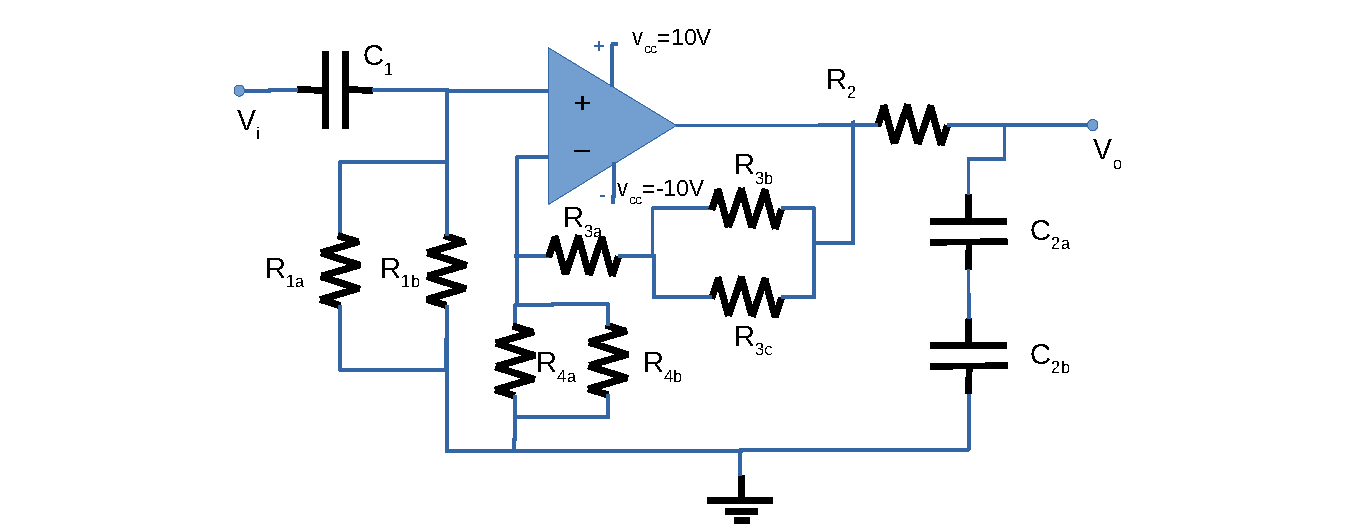
\includegraphics[width=0.8\linewidth]{circuit.pdf}
\caption{Band Pass Filter Circuit}                                     
\label{fig:circuit}
\end{figure}
This circuit is composed by 5 resistors, 2 capacitors and an OPAMP.
The values of the components are exhibited in the table below.
\begin{table}[H]
  \centering
  \begin{tabular}{|l|r|}
     \hline    
    {\bf Name} & {\bf Value} \\ \hline   
    $R_{1a}$ & 1.000000e+03 Ohm \\ \hline
$R_{1b}$ & 1.000000e+04 Ohm \\ \hline
$R_{1}$ & 9.090909e+02 Ohm\\ \hline
$R_{2}$ & 1.000000e+03 Ohm \\ \hline
$R_{3a}$ & 1.000000e+05 Ohm \\ \hline
$R_{3b}$ & 1.000000e+05 Ohm \\ \hline
$R_{3c}$ & 1.000000e+05 Ohm \\ \hline
$R_{3}$ & 1.500000e+05 Ohm \\ \hline
$R_{4a}$ & 1.000000e+03 Ohm \\ \hline
$R_{4b}$ & 1.000000e+04 Ohm \\ \hline
$R_{4}$ & 9.090909e+02 Ohm \\ \hline
$C_{1}$ & 2.200000e-07 F \\ \hline
$C_{2a}$ & 2.200000e-07 Ohm \\ \hline
$C_{2b}$ & 2.200000e-07 Ohm \\ \hline
$C_{2}$ & 1.100000e-07 F \\ \hline

  \end{tabular}
  \caption{Components Values}
  \label{tab:datags}
\end{table}

In Section~\ref{sec:analysis}, a theoretical analysis of the circuit, 
performed on Octave, is presented. In Section~\ref{sec:simulation}, the 
circuit is analysed by simulation, using NGSpice, and the results are compared to 
the theoretical results obtained in Section~\ref{sec:analysis}. The conclusions 
of this study are outlined in Section~\ref{sec:conclusion}.

